\documentclass[letterpaper,12pt]{report}
\usepackage[top=1in, bottom=1in, left=1in, right=1in]{geometry}
\usepackage{fancyhdr,tocloft,natbib,url,graphicx,float,listings,sidecap,wrapfig}
\usepackage[font=small,labelfont=bf,labelsep=period]{caption}
\usepackage{tabularx}
\usepackage{setspace}
\usepackage{hyperref}
\usepackage[all]{hypcap}
\usepackage{qtree,algorithm,algorithmic}
\pagestyle{plain}
\fancyhf{}
\lhead{}
\chead{}
\rhead{}
\cfoot{\thepage}


%\floatstyle{boxed}
%\restylefloat{figure}

\hypersetup {
	colorlinks=false,
	pdfborder={0 0 0},
}

\setcounter{secnumdepth}{3}
\renewcommand*\thesection{\arabic{section}.}
\renewcommand*\thesubsection{\thesection \arabic{subsection}.}
\renewcommand*\thesubsubsection{\thesubsection \arabic{subsubsection}.}

\setcounter{tocdepth}{3}
\renewcommand\contentsname{}				% TOC title
\renewcommand\listfigurename{}				% LOF title
\renewcommand\listtablename{}				% LOT title
\setlength\cftaftertoctitleskip{-0.5in}
\setlength\cftafterloftitleskip{-0.5in}
\setlength\cftafterlottitleskip{-0.5in}

\renewcommand\bibsection{\section{References}}

\begin{document}

\hypersetup{pageanchor=false}
%%  COVER PAGE
\begin{titlepage}
	\begin{center}
		\vspace*{0.5in}
		\begin{doublespace}
			\LARGE \textbf{Immersive Quiz for Spanish Learners} \\
			\vspace*{1in}
			\normalsize
			A Manuscript \\
			Submitted to \\
			the Department of Computer Science \\
			and the Faculty of the\\
			University of Wisconsin--La Crosse \\
			La Crosse, Wisconsin \\
			\vspace*{0.5in}
			by \\
			\large
			\textbf{Austin Klum} \\

			\vspace*{0.5in}
			\normalsize
			in Partial Fulfillment of the \\
			Requirements for the Degree of\\
			\Large{\textbf{Master of Software Engineering}} \\
			\normalsize
			May, 2022
		\end{doublespace}
	\end{center}
\end{titlepage}
	
\clearpage

%% SIGNATURE PAGE
\thispagestyle{empty}
\vspace*{0.3in}
\begin{center}
	\large{\textbf{Immersive Quiz for Spanish Learners}} \\ 
	\vspace{0.75in}
	\normalsize{By Austin Klum}
\end{center}

\vspace{0.5in}
\noindent We recommend acceptance of this manuscript in partial fulfillment of this candidate's requirements for the degree of Master of Software Engineering in Computer Science. The candidate has completed the oral examination requirement of the capstone project for the degree. \\

\noindent
\begin{tabularx}{\textwidth}{p{3in}Xp{2in}}
		\rule{0pt}{50pt} & & \\
	\hrulefill & & \hrulefill \\
	Prof. Elliott Forbes & & Date \\
	Examination Committee Member & & \\
	\rule{0pt}{50pt} & & \\
	\hrulefill & & \hrulefill \\
	Prof. Thomas Gendreau & & Date \\
	Examination Committee Member & & \\
	\rule{0pt}{50pt} & & \\
	\hrulefill & & \hrulefill \\
	Prof. Dipankar Mitra & & Date \\
	Examination Committee Member & & \\
\end{tabularx}


\clearpage

\hypersetup{pageanchor=true}
\setcounter{page}{1}
\pagenumbering{roman}
\renewcommand\arraystretch{1.5}

%% ABSTRACT
\section*{Abstract}
\addcontentsline{toc}{section}{Abstract}
Austin Klum, J., ``Immersive Quiz for Spanish Learners,'' Master of Software Engineering, May 2021, (Elliot Forbes, Ph.D.). \\

This manuscript describes the development of a virtual reality tool to provide an immersive quiz taking experience for Spanish learners. Virtual reality is  
\clearpage

%%% ACKNOWLEDGEMENTS
\section*{Acknowledgements}
\addcontentsline{toc}{section}{Acknowledgments}
I would like to express my sincere appreciation to my project advisor Dr. Kasi Periyasamy for his invaluable guidance and untiring support. I would also like to express my thanks to the Department of Computer Science at the University of Wisconsin--La Crosse for providing the learning materials and computing environment for my project.
\clearpage

%% TABLE OF CONTENTS
\section*{Table of Contents}
\tableofcontents
\clearpage


%% LIST OF TABLES
\section*{List of Tables}
\addcontentsline{toc}{section}{List of Tables}
\listoftables
\clearpage

%% LIST OF FIGURES
\section*{List of Figures}
\addcontentsline{toc}{section}{List of Figures}
\listoffigures
\clearpage

%% GLOSSARY
\section*{Glossary}
\addcontentsline{toc}{section}{Glossary}
\subsection*{ASP.NET Core}

Lorem ipsum

\subsection*{ASP.NET Core MVC}
Lorem ipsum
\subsection*{Unity}
Lorem ipsum
\subsection*{Unity XR}
Lorem ipsum
\subsection*{\C}
Lorem ipsum
\subsection*{LINQ}
Lorem ipsum
\subsection*{Entity Framework Core}
Lorem ipsum
\subsection*{SQL Server}
Lorem ipsum
\subsection*{Transparent Date Encryption (TDE)}
Lorem ipsum
\subsection*{Basic Authentication}
Lorem ipsum
\subsection*{JSON}
Lorem ipsum
\subsection*{HTTPS}
Lorem ipsum
\subsection*{REST}
Lorem ipsum
 \subsection*{CSS}
Lorem ipsum
\subsection*{HTML}
Lorem ipsum
\subsection*{Bootstrap}
Lorem ipsum
\subsection*{Web API}
Lorem ipsum
\subsection*{GUID}
Lorem ipsum
\subsection*{Git}
Lorem ipsum
\subsection*{Dependency Injection}
Lorem ipsum
\subsection*{Razor View Engine}
Lorem ipsum
\subsection*{Visual Studio}
Lorem ipsum
\subsection*{Unity Editor}
Lorem ipsum


\clearpage

\setcounter{page}{1}
\pagenumbering{arabic}

\IfFileExists{section01/section}{\section{Introduction}
\label{sec:Introduction}

\subsection{Overview} 
This gives a brief overview of this section.

\subsection{Point 1}
This subsection gives a great deal of precise description supporting point 1.  For example,
Figure \ref{State Chart} explains in great detail a \index{state chart}state chart.

\begin{figure}[htb]
\centering
\includegraphics[width=.5\textwidth]{section01/assets/sample_image.png}
\caption[Short Caption]{\label{State Chart}State Chart Diagram}
\end{figure}

\subsection{Point 2}
This gives Point 2
}{}\clearpage
\IfFileExists{section02/section}{\section{Requirements}
\label{sec:Requirements}

\subsection{Overview} 
This gives a brief overview of this section.

\subsection{Point 1}
This subsection gives a great deal of precise description supporting point 1.  For example,
Figure \ref{State Chart 2} explains in great detail a state chart.

\begin{figure}[htb]
\centering
\includegraphics[width=.5\textwidth]{section02/assets/sample_image.png}
\caption[Short Caption 2]{\label{State Chart 2}State Chart Diagram}
\end{figure}

\subsection{Point 2}
This gives Point 2
}{}\clearpage
\IfFileExists{section03/section}{\section{Design and Implementation}
\label{sec:DesignImplementation}

\subsection{Overview} 
This gives a brief overview of this section.

\subsection{Point 1}
This subsection gives a great deal of precise description supporting point 1.  For example,
Figure \ref{State Chart 3} explains in great detail a state chart.

\begin{figure}[htb]
\centering
\includegraphics[width=.5\textwidth]{section03/assets/sample_image.png}
\caption[Short Caption 3]{\label{State Chart 3}State Chart Diagram}
\end{figure}

\subsection{Point 2}
This gives Point 2
}{}\clearpage

%% BIBLIOGRAPHY
\section{Bibliography}
\label{sec:bibliougraphy}
\clearpage

%%% APPENDICES
\section{Appendices}
\label{sec:appendices}
\clearpage

\end{document}
